\subsection{Macchina a Stati}
È un grafo "\emph{stati-transizioni}" che permette di descrivere il comportamento delle istanze di una classe.
A differenza dei \emph{diagrammi delle attività} dove l'obbiettivo è mettere in ordine un insieme di azioni, qui viene
mostrata l'evoluzioni degli oggetti in risposta a determinati eventi.
\newline\newline
Ogni \textcolor{cyan}{transizione} avviene al verificarsi di un determinato evento interno, rappresentato da un'\emph{operazione}
della classe; oppure tramite messaggi inviati da altri oggetti.

In una \emph{transizione}, gli \emph{\textcolor{cyan}{eventi}} possono essere accompagnati
anche da una \emph{\textcolor{cyan}{condizione}} e da una sequenza di azioni.

\begin{figure}[h]
    \centering
    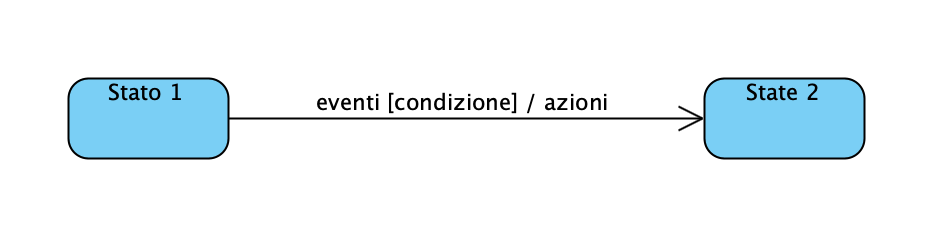
\includegraphics[scale=0.7]{img/machinediagram.png}
\end{figure}

La semantica è la seguente: se si verifica almeno uno degli eventi, e vale la condizione, si eseguono
tutte le azioni e si passa nell'altro stato.

\subsubsection{Eventi}

Le \emph{transizioni} possono essere \emph{non deterministiche}, cioè da uno stato ci possono
essere più transizioni con lo stesso evento.

Gli eventi possono classificarsi in:
\begin{itemize}
    \item Eventi di \textcolor{cyan}{operazione} o \textcolor{cyan}{segnale}: \verb|op(a: T)|. Ovvero la transizione
        è abilitata quando riceve un segnale o avviene una chiamata di metodo con parametri \verb|a| e tipo \verb|T|.
    \item Eventi di \textcolor{cyan}{variazione}: \verb|when(exp)|. La transizione è abilitata quando \verb|exp| diventa vera.
    \item Eventi \textcolor{cyan}{temporali}: \verb|after(time)|. La transizione è abilitata dopo che l'oggetto è stato fermo per
        un tempo \verb|time| in quello stato.
\end{itemize}

\paragraph{\textcolor{cyan}{Entry}} Anche chiamata \emph{azione di entrata}, viene eseguita all'ingresso di uno stato.
\paragraph{\textcolor{cyan}{Exit}} Anche chiamata \emph{azione di uscita}, viene eseguita quando si esce da uno stato.
\paragraph{\textcolor{cyan}{Transizione Interna}} Risposta a un determinato evento, ma si rimane nello stesso stato.
\paragraph{\textcolor{cyan}{Do-Activity}} Azione eseguita in continuazione finchè l'oggetto si trova in quello stato.
A differenza delle altre \emph{azione} che sono \emph{atomiche}, queste consumano del tempo e possono essere interrotte, ad esempio
quando si esce dallo stato.

\begin{figure}[h]
    \centering
    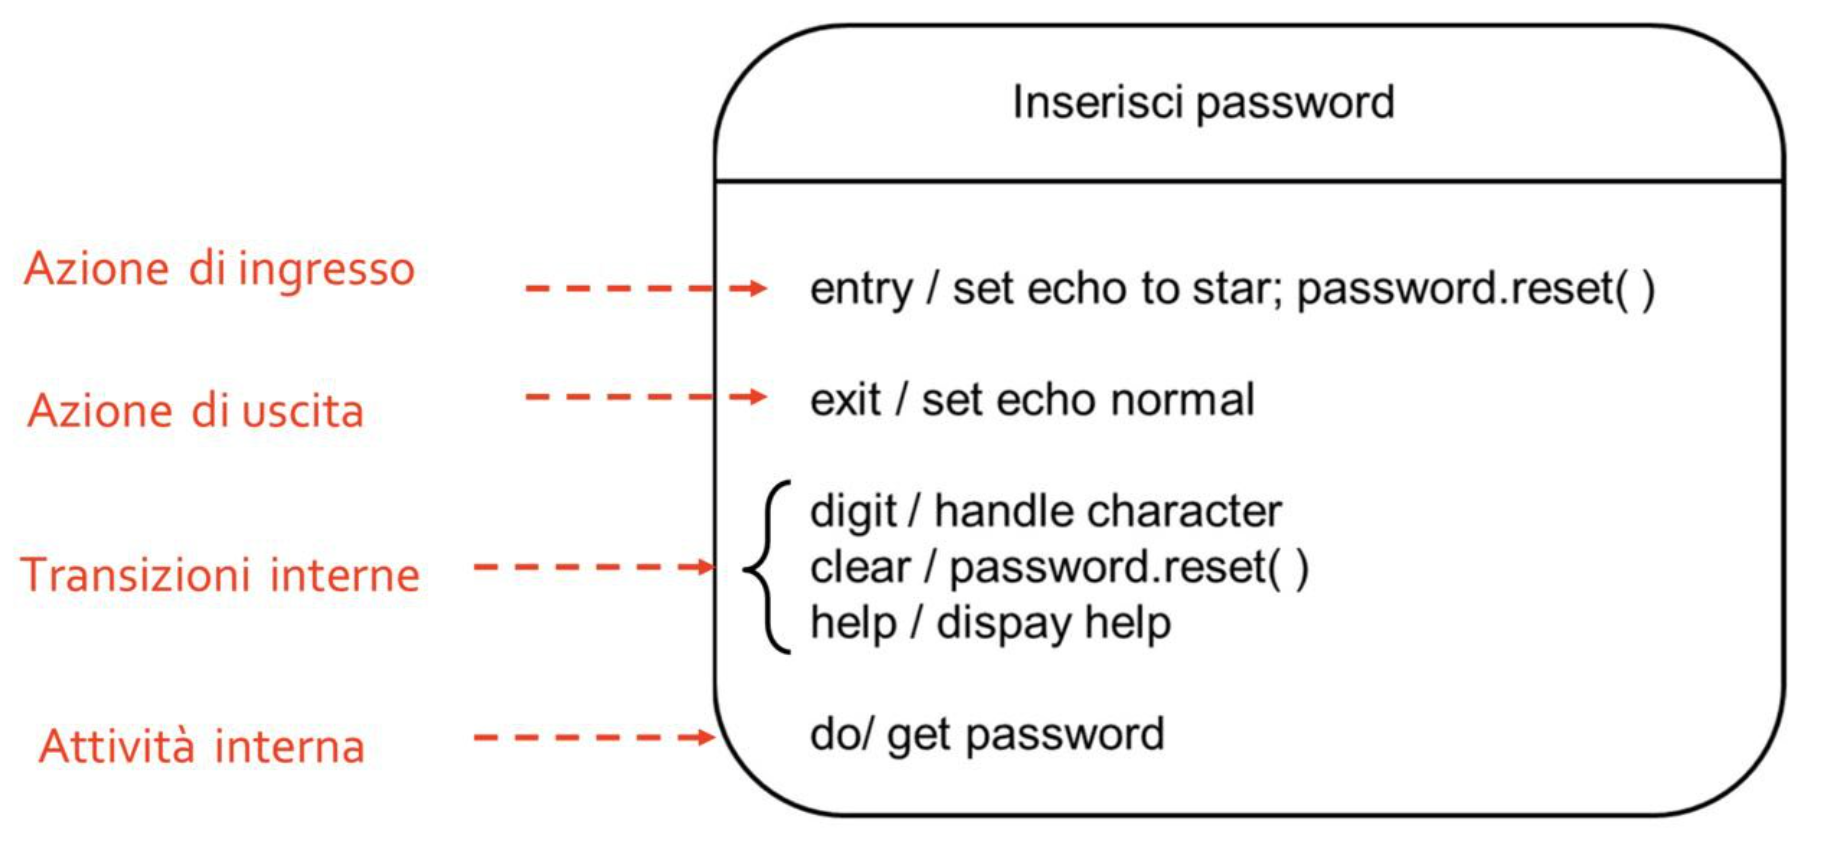
\includegraphics[scale=0.37]{img/entry.png}
\end{figure}

\newpage

\subsubsection{Stato Composito Sequenziale}
Consiste nell'avere uno stato che contiene un'altra \emph{macchina a stati}.
Quando una transizione entrante nello \emph{\textcolor{cyan}{stato composito}} termina sul bordo, vuol
dire che si prosegue a partire dallo \emph{stato iniziale} dello \emph{stato composito}. Altrimenti la transizione
può avere come \emph{target} anche uno stato interno.
Le transizioni di uscita, invece, possono anch'esse partire dal bordo, in tal caso
significa che ci si può andare da qualsiasi stato interno, altrimenti quelle che partono da un singolo stato interno
sono possibili solo da esso. Esiste anche una transizione d'uscita speciale chiamata di \textcolor{cyan}{completamento},
dalla quale ci si può passare solo una volta arrivati nello stato finale dello stato composito.

\begin{figure}[H]
    \captionsetup{justification=centering}
    \centering
    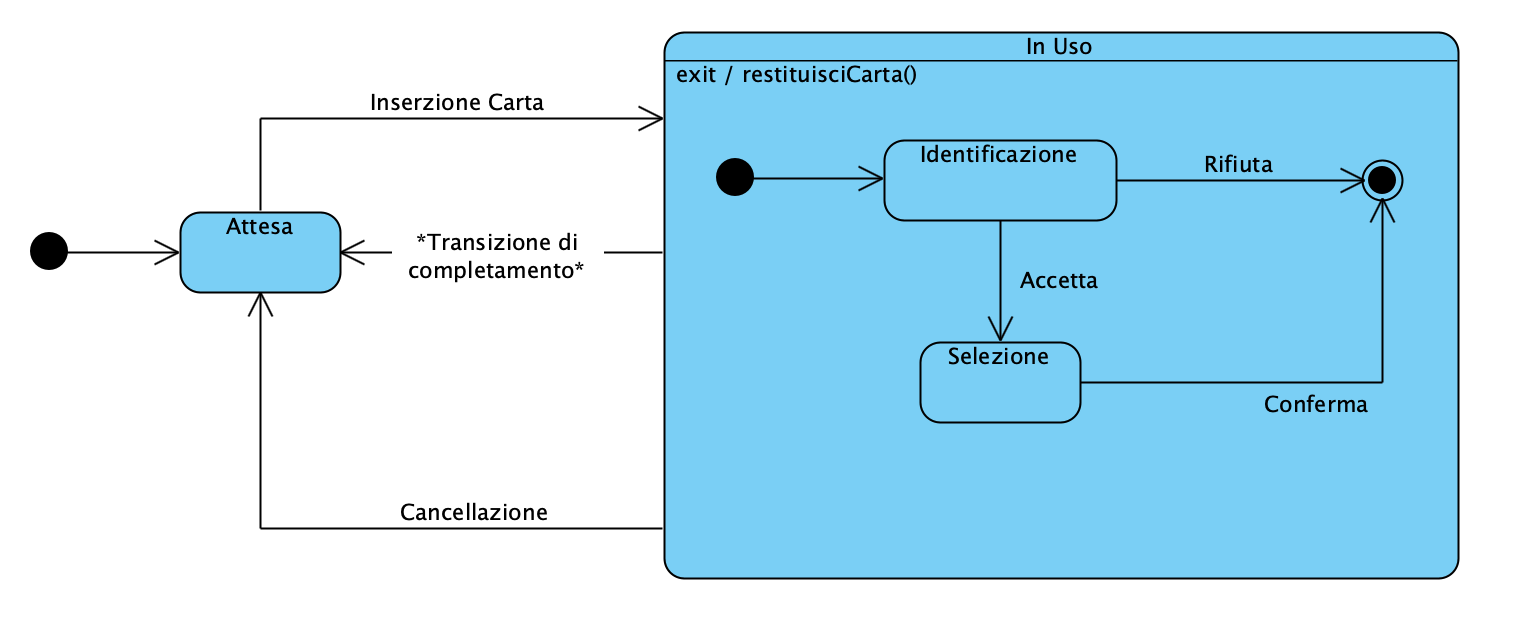
\includegraphics[scale=0.45]{img/statocompositoseq.png}
    \caption{Esempio di macchina a stati che descrive l'uso di un sistema di pagamento con stato composito sequenziale.}
\end{figure}

\newpage

\subsubsection{Stato Composito Parallelo}
Nello \emph{stato composito} abbiamo più sottostati che si eseguono in modo
parallelo. Una transizione entrante sul bordo attiva tutti gli stati iniziali.
La \emph{transizione di completamento} può avvenire solo se si è arrivati in tutti gli stati finali.
Mentre, una transizione di uscita che parte dal bordo è raggiungibile da un qualunque stato interno e fà uscire da \textbf{tutti}
i sottostati. Anche un transizione che parte da un singolo stato interno fà uscire da tutti i sottostati e può avvenire solo se ci
si trova in quel determinato stato.

\begin{figure}[H]
    \centering
    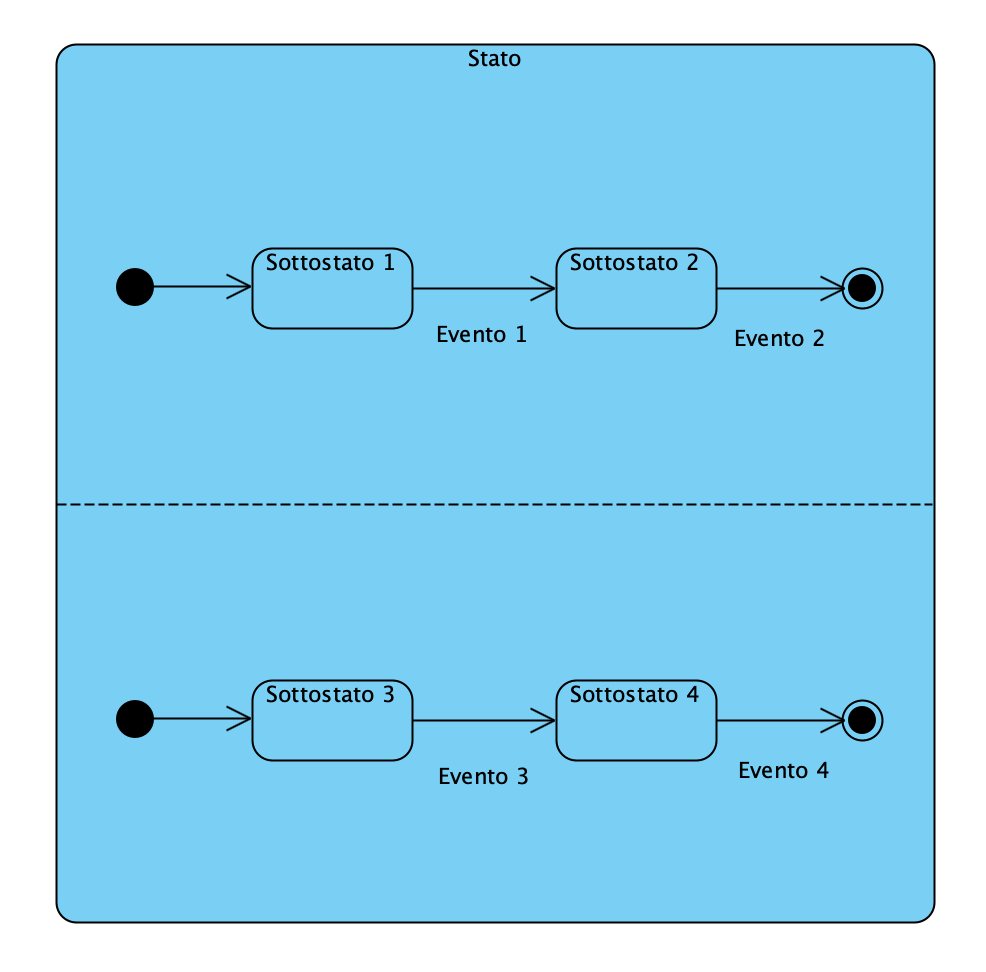
\includegraphics[scale=0.6]{img/statoparallelo.png}
\end{figure}

\subsubsection{Sottomacchine}
Le \textcolor{cyan}{sottomacchine} si usano quando si vuole rappresentare
uno stato composito in un diagramma a parte, in modo da poterlo riusare in più contesti.
La \emph{sottomacchina} ha un nome che ne definisce il \verb|Tipo| e le sue istanze
si indicano con \verb|Nome Istanza: Tipo|.

\paragraph{\textcolor{cyan}{Entry \& Exit Points}} Sono dei nodi che servono per poter collegare le transizioni
della macchina principale con la sottomacchina.

\begin{figure}[H]
    \centering
    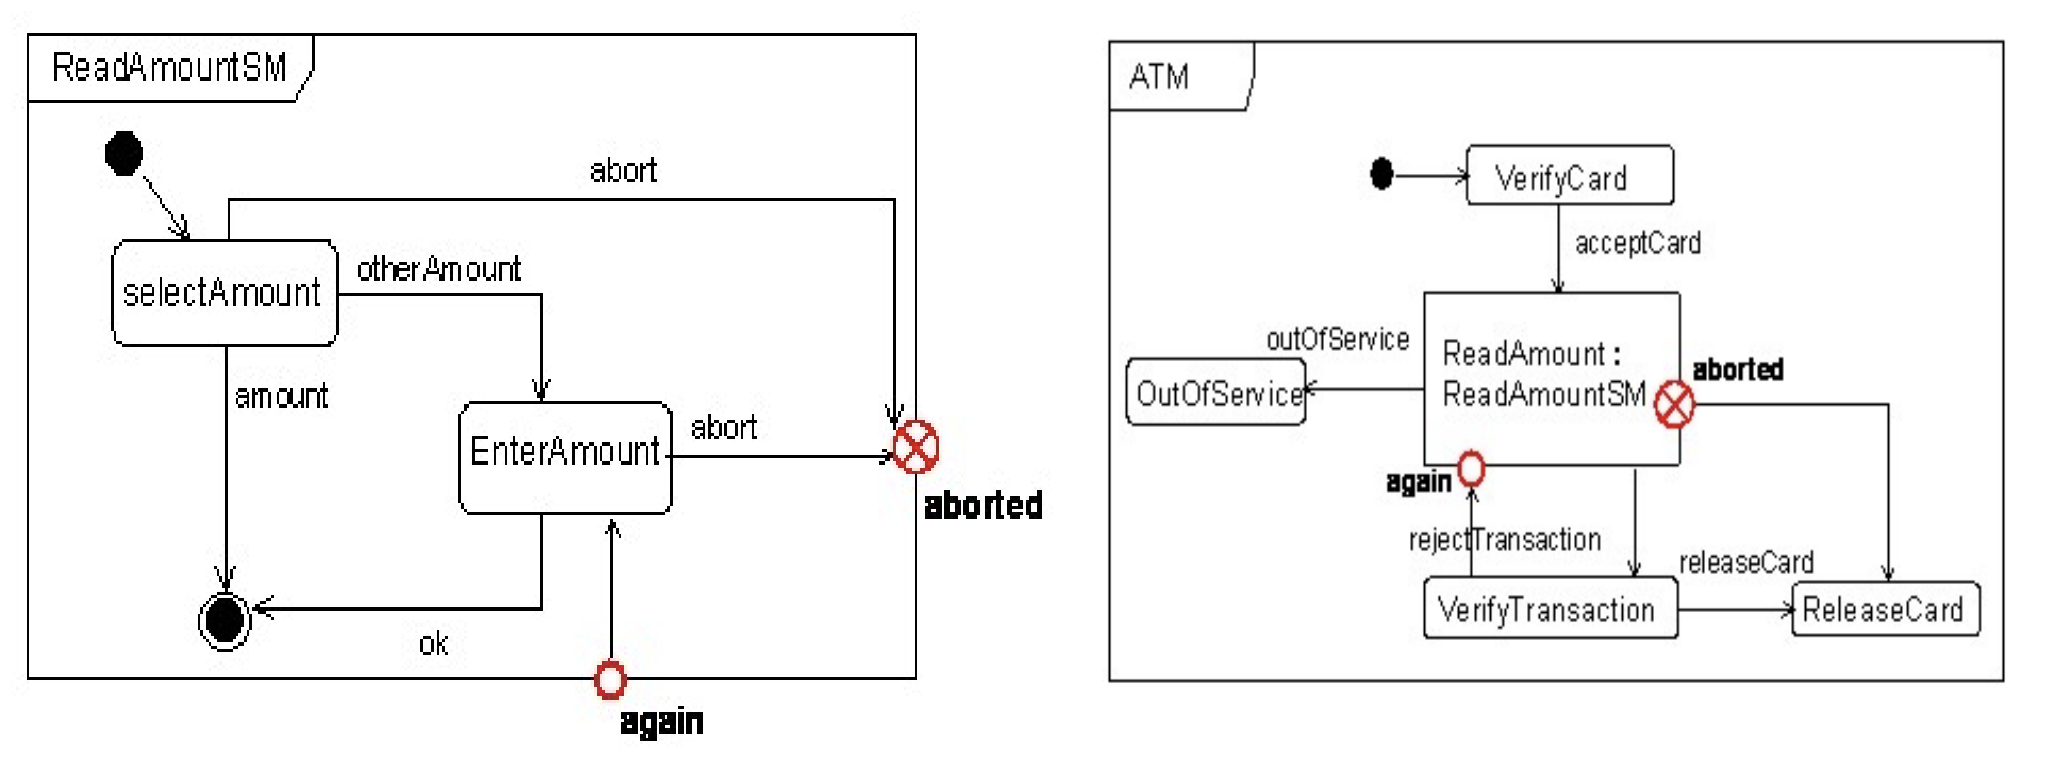
\includegraphics[scale=0.33]{img/sottomacchine.png}
\end{figure}

In questo caso le \emph{transizioni di completamento} possono scattare anche quando si arriva in un \emph{exit point}. 

\subsubsection{Pseudostati}

\paragraph{\textcolor{cyan}{Giunzione}} Uno \emph{pseudostato} da cui possono entrare e/o uscire due o più transizioni.
Se sono presenti condizioni, queste sono valutate in modo \textcolor{cyan}{statico}, quindi prima che avvengano gli eventi interessati.
Inoltre, se le condizioni non coprono tutti i casi, l'evento può essere ignorato e si rimane in quello stato.

\begin{figure}[H]
    \centering
    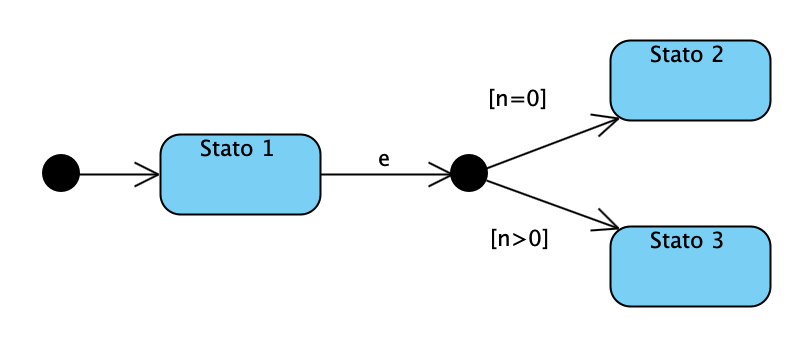
\includegraphics[scale=0.7]{img/giunzione.png}
\end{figure}

\paragraph{\textcolor{cyan}{Decisione}}

A differenza delle \emph{\textcolor{cyan}{giunzioni}}, questo sono valutate \textcolor{cyan}{dinamicamente}, quindi dopo che avvengono
gli eventi; e devono coprire tutti i casi possibili. Ovviamente un'altra differenza con le \emph{giunzioni} è che in questo caso la transizione
entrante può essere solo \underline{una}.

\begin{figure}[H]
    \captionsetup{justification=centering}
    \centering
    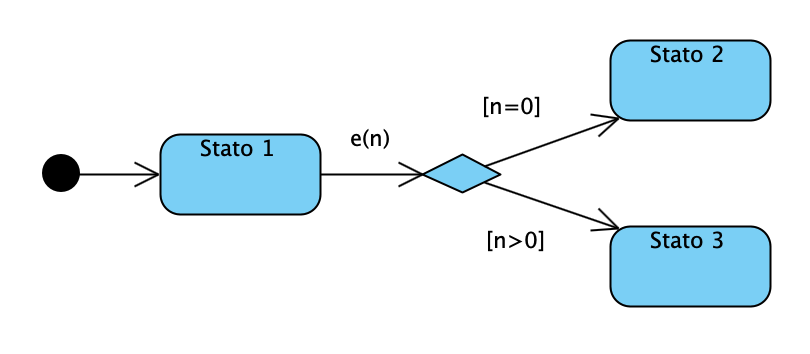
\includegraphics[scale=0.7]{img/choice.png}
    \caption{In questo esempio bisogna avere garanzia che $n \geq 0$.}
\end{figure}

\paragraph{\textcolor{cyan}{Storia}}

Lo stato \emph{\textcolor{cyan}{history}} permette di memorizzare lo stato della macchina
quando viene \emph{interrotta} o \emph{spenta}. La transizione entrante nello stato \emph{history}, invoca il
ripristino dello stato precedente, mentre se c'è una transizione uscente, questa indica lo stato in cui passare nel caso
in cui la macchina non sia ancora stata mai interrotta, quindi quando lo stato \emph{history} è vuoto.

\begin{figure}[H]
    \captionsetup{justification=centering}
    \centering
    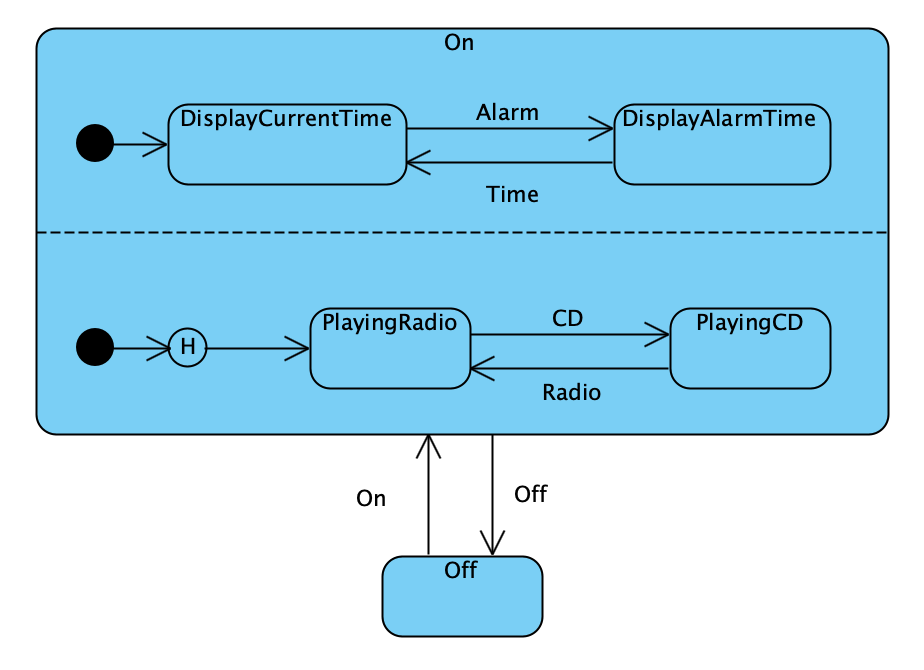
\includegraphics[scale=0.7]{img/history.png}
    \caption{In questo esempio di funzionamento di un autoradio, la prima volta che si accenderà verrà riprodotta in automatico una stazione radio.}
\end{figure}